\documentclass{bioinfo}
\usepackage{color}
\usepackage{listings}
\lstset{ 
basicstyle=\ttfamily,       % the size of the fonts that are used for the code
                  % how far the line-numbers are from the code
backgroundcolor=\color{white},  % choose the background color. You must add \usepackage{color}
showspaces=false,               % show spaces adding particular underscores
showstringspaces=false,         % underline spaces within strings
showtabs=false,                 % show tabs within strings adding particular underscores
frame=single,           % adds a frame around the code
tabsize=2,          % sets default tabsize to 2 spaces
captionpos=b,           % sets the caption-position to bottom
breaklines=true,        % sets automatic line breaking
breakatwhitespace=false,    % sets if automatic breaks should only happen at whitespace
escapeinside={\%*}{*)}          % if you want to add a comment within your code
}
\copyrightyear{2005}
\pubyear{2005}

\begin{document}
\firstpage{1}

\title[Application Note]{Supplementary for bioWeb3D: an online webGL 3D data visualisation tool}
\author[Pettit \textit{et~al}]{Jean-Baptiste Pettit\,$^{*}$ and John C. Marioni$^{*}$}
\address{EMBL-EBI, European Molecular Biology Laboratory - European Bioinformatics Institute, Cambridge, CB10 1SD, UK}

\history{Received on XXXXX; revised on XXXXX; accepted on XXXXX}

\editor{Associate Editor: XXXXXXX}

\maketitle
\section{Input file formats}
\subsection{Dataset files}

\vbox{When the user adds a new {\it{Dataset}} file, a new Dataset section is created in the ``Data" panel of the application. One raw data file contains one dataset. The dataset is composed only of 3D coordinates (x,y,z) along with a small amount of additional information (e.g., an optional name, an optional ``chain" that has to be set to true to link the points together). Below is an example of a minimal 3 point dataset file:
\begin{lstlisting}
{ "dataset" : {
      "name" : "my superb dataset",
      "chain" : true,
       points" :
        [
          [
            0.5,
            100,
            -50.5
          ],
          [
            200,
            10,
            0.0
          ],
          [
            3,
            250.15,
            15
          ]
        ]
     }
}
\end{lstlisting}}

\subsection{Information layer files}

The {\it{Information layer}} file contains information about the points described in the Dataset file. The information entered in this file has to be inputted in the same order as the points defined in the Dataset file. Multiple information layers can be defined in the same file as follows:
\begin{itemize}
\item{a name}
\item{a number of categories called numClass}
\item{A list of labels for the classes (optional)}
\end{itemize}
For example coming back to the 3 points defined previously, two information layers could correspond to: 
\begin{itemize}

\item{one clustering algorithm that puts the first two points together in class one and the third point alone in a second class}
\item{a second clustering algorithm that puts each point in a separate class}
\end{itemize}

In this case the Information layer file would look like:

\vbox{
\begin{lstlisting}
{ "information" :
  [
    {
      "name": "clustering algo 1",
      "numClass": "2",
      "labels" : [
        "Category 1",
        "Category 2"
      ],
      "values": [
        1,
        1,
        2
      ]
    },
    {
      "name": "clustering algo 2",
      "numClass": "3",
      "values": [
        1,
        2,
        3
      ]
    }
  ]
}
\end{lstlisting}}

\section{Converting CSV files to Json}
Much data generated in the biological sciences is stored within CSV files. Converting CSV document to the JSON format used in this application is not always trivial. In order to facilitate this process, we provide scripts written in Perl to perform the conversion. We describe hereafter the CSV formats handled by the converters.
\subsection{CSV to dataset file}
To use the ``csv\_to\_dataset.pl" converter, the input CSV file must contain only the points coordinates. Each line represents a point and the three coordinates on each line must be separated by ``tabulation" characters. Example :
\begin{lstlisting}
0.5	100	-50.5
200	10	0.0
3	250.15	15
\end{lstlisting}
The syntax to use the converter is the following :
\begin{lstlisting}
perl csv_to_dataset.pl [csv file] [dataset name] [Chain parameter : true if the points should be linked, false otherwise]
\end{lstlisting}
For example, if the previous CSV file is named ``example.csv", and the points should be linked, then the command line will be:
\begin{lstlisting}
perl csv_to_dataset.pl example.csv my_dataset true
\end{lstlisting}
The result file named ``example.csv.json" will contain :
\begin{lstlisting}
{ "dataset" : {
      "name" : "my_dataset",
      "chain" : true,
        "points" : [
          [
            0.5,
            100,
            -50.5
          ],
          [
            200,
            10,
            0.0
          ],
          [
            3,
            250.15,
            15
          ]
        ]
     }
}
\end{lstlisting}

\subsection{CSV to information layer file}
To use the ``csv\_to\_information\_layer.pl" converter, each column of the CSV file should contain one information layer. The first element of each column will be the name of the information layer, and the rest of the column represents in which class each point belongs. The separation character between columns must be a ``tabulation". for example :
\begin{lstlisting}
clustering_algo_1	clustering_algo_2
1	1
1	2
2	3
\end{lstlisting}
The syntax to use the converter is the following :
\begin{lstlisting}
perl csv_to_information_layer.pl [csv file]
\end{lstlisting}
For example if, the previous CSV file is named ``example\_information\_layer.csv", then the command line will be:
\begin{lstlisting}
perl csv_to_information_layer.pl example_information_layer.csv
\end{lstlisting}
The result file named ``example\_information\_layer.csv.json" will contain :
\begin{lstlisting}
{ "information" :
  [
    {
      "name": "clustering_algo_1",
      "numClass": "2",
      "values": [
        1,
        1,
        2
      ]
    },
    {
      "name": "clustering_algo_2",
      "numClass": "3",
      "values": [
        1,
        2,
        3
      ]
    }
  ]
}
\end{lstlisting}
Please note that at the moment it is not possible to use the ``labels" property with this converter. 
\section{further examples}
\subsection{Visualizing simultaneous worlds}
You can choose to split the application screen in up to 4 different worlds in order to visualize and compare different information layers of the same dataset or different datasets (figure \ref{fig:01}).
\begin{figure}[h!]%figure1
\centerline{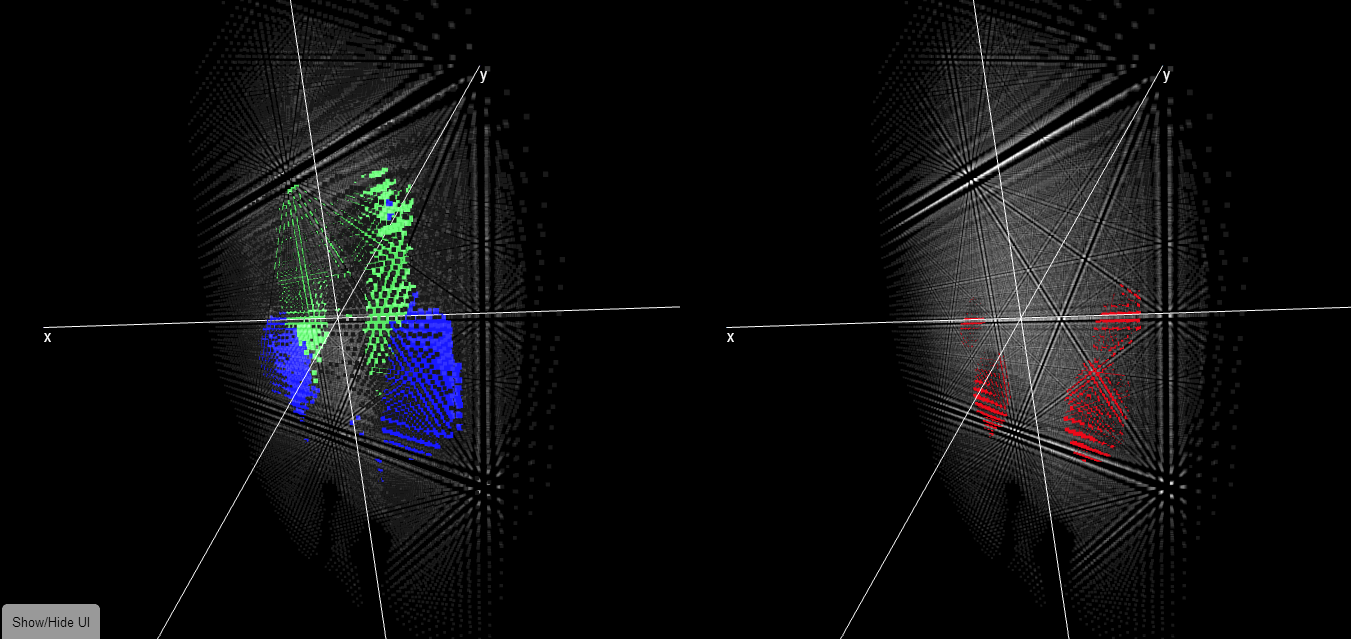
\includegraphics[totalheight=0.19\textheight]{Supp_fig1.png}}
\caption{In this figure, the left-hand world shows two clusters (in blue and green) in the brain of the marine annelid {\it Platynereis dumerilii} and the right-hand world shows the expression data for the gene C-Opsin (in red) in the same dataset. Data for this figure was taken from \citep{Tomer10}.}\label{fig:01}
\end{figure}
\subsection{Visualizing sequential information}
If the ``chain" property in the dataset file is set to ``true", the point will be linked together in the 3D visualization (figure \ref{fig:02}).
\begin{figure}[h!]%figure1
\centerline{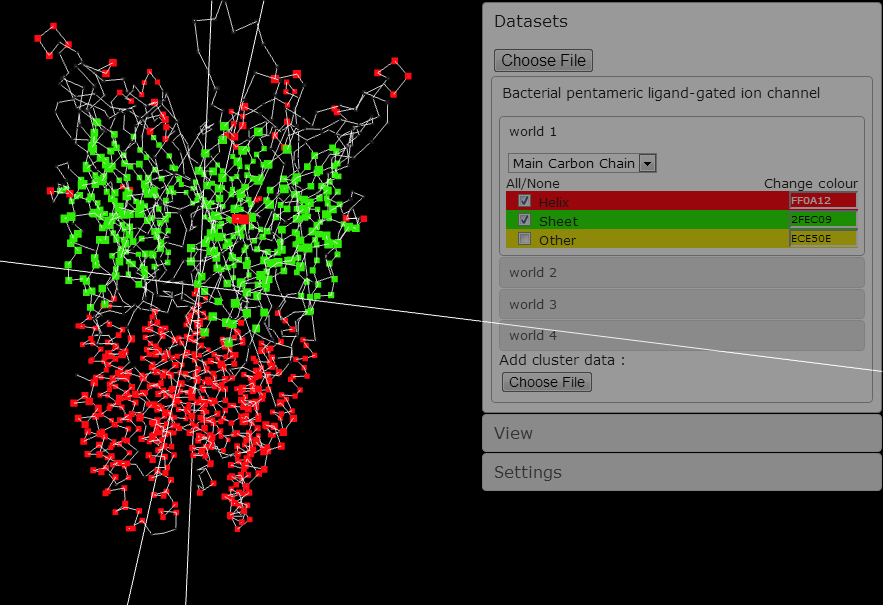
\includegraphics[totalheight=0.2\textheight]{Supp_fig2.png}}
\caption{An example of a sequential dataset where the points are linked together. Here we present the 3D structure of the main carbon chain of a bacterial pentameric ligand-gated ion channel. In red we show the carbon atoms which are part of an $\alpha$-helix secondary structure, in green we show the atoms which are part of a $\beta$-sheet secondary structure. Data for this figure was taken from the Protein Data Bank in Europe website}\label{fig:02}
\end{figure}
\begin{thebibliography}{}
\bibitem[Tomer {\it et~al}., 2010]{Tomer10} Tomer R., Denes A.S., Tessmar-Raible K., Arendt D. (2010). Profiling by image registration reveals common origin of annelid mushroom bodies and vertebrate pallium. {\it{Cell}}, {\bf{142}}:800-809. 
\end{thebibliography}
\end{document}
